\apendice{Especificación de diseño}

\section{Introducción}

En esta sección se explicará la estructura de los datos de la aplicación, así como de su arquitectura y su funcionamiento.

\section{Diseño de datos}
Un aspecto a tener en consideración en cuanto a la estructura de los datos es que no estamos utilizando una base de datos relacional, y por tanto no contamos con una estructura de tablas. Neo4j es una base de datos NoSQL orientada a grafos, por tanto la 2 entidades con la que estructurar la base de datos son los nodos y enlaces. Ambas entidades cuentan con etiquetas propias para poder identificar su tipo. Explicaré todas aquellas utilizadas en este trabajo.

\subsection{Nodos}

En cuanto a nodos de la base de datos contamos con principales etiquetas \texttt{:Place} para los lugares y \texttt{:Category} para las categorías.

\subsubsection{\texttt{:Place}}

Los nodos con esta etiqueta son cada una de las ubicaciones obtenidas de OpenStreetMap. Cuenta con los siguientes atributos:

\begin{itemize}
	\item \texttt{area}: \textit{String} con el nombre de la ciudad a la que pertenecen.
	\item \texttt{category}: \textit{String} con el nombre de la categoría comercial a la que pertenece,
	\item \texttt{coords}: Tipo \textit{Point} de Neo4j con las coordenadas de la ubicación.
	\item \texttt{id}: \textit{Integer} con el número identificativo de la ubicación en OpenStreetMap
	\item \texttt{type}: \textit{String} identificativo de si la categoría de este nodo pertenece a \textit{amenity} o \textit{shop}.
	\item \texttt{Q}: JSON serializado en formato \textit{String} que contiene los índices de calidad para dicha ubicación.
\end{itemize}

Los campos anteriores son los que están presentes en todos los nodos de este tipo. Algunos nodos contienen atributos adicionales con la información que OpenStreetMap provee para dicha ubicación, estos pueden ser nombre, teléfono, página web, entre otros.

\subsubsection{\texttt{:Category}}
Estos nodos son los constitutivos de la red de categorías de cada ciudad. Cada una estará compuesta por las categorías presentes únicamente en esa ciudad.

Cada nodo posee los siguientes atributos:

\begin{itemize}
	\item \texttt{city}: \textit{String} con la ciudad a la que pertenece dicha categoría.
	\item \texttt{n\_nodes}: \textit{Integer} con el número de nodos que posee dicha categoría en esa ciudad.
	\item \texttt{name}: \textit{String} con el nombre de la categoría comercial.
	\item \texttt{type}: \textit{String} con el tipo de categoría entre \textit{amenity} y \textit{shop}
\end{itemize}

\subsubsection{\texttt{:User}}
Si bien los usuarios no juegan un papel importante en comparación a las otras entidades estos también deben de contar con una representación en la base de datos.

Cuentan con los siguientes atributos:

\begin{itemize}
	\item \texttt{userId}: \textit{String} con UUID identificativo del usuario.
	\item \texttt{user\_name}: \textit{String} con el nombre de usuario.
	\item \texttt{password}: \textit{String} con la contraseña cifrada del usuario.
	\item \texttt{name}: \textit{String} con el nombre personal del usuario.
	\item \texttt{surname}: \textit{String} con el apellido del usuario.
	\item \texttt{role}: \textit{String} con el rol del usuario.
	\item \texttt{mail}: \textit{String} con correo electrónico del usuario.
\end{itemize}

\subsection{Enlaces}
La otra entidad con la que contamos en la base de datos son los enlaces. Estos más allá de servir como simple enlace entre nodos, también pueden almacenar atributos además de poder asignarles etiquetas identificativas.

\subsubsection{\texttt{:IS\_NEAR}}
Este tipo de enlaces son aquellos representativos de la proximidad entre ubicaciones comerciales. Al igual que se indicaba en la memoria, estos se crean únicamente entre nodos con una distancia entre sí menor o igual a 100 metros.

Cuentan con un único atributo de nombre \texttt{distance} de tipo \textit{Float} con la distancia entre los dos nodos enlazados.

Este tipo de enlace solo une nodos etiquetados como \texttt{:Place}.

\subsubsection{\texttt{:Rel}}
Estos enlaces son representativos de las interacciones entre categorías. Dado que necesitamos contar con la matriz de interacción, la red de categorías tendrá un subgrafo compuesto por los nodos categoría de una ciudad y con enlaces de este tipo conectando cada par de estos nodos.

Cada uno de estos enlaces tiene los siguientes atributos:
\begin{itemize}
	\item \texttt{real\_value}: \textit{Integer} con el valor real de interacción entre el par de categorías.
	\item \texttt{a\_ij}: \textit{Float} con el valor de la matriz de coeficientes del método \textit{Permutation}.
	\item \texttt{perc\_25}: \textit{Float} con el valor del percentil 0.25 de las simulaciones.
	\item \texttt{perc\_975}: \textit{Float} con el valor del percentil 0.975 de las simulaciones.
	\item \texttt{std\_dev}: \textit{Float} con el valor de la desviación estandar de las simulaciones.
	\item \texttt{mean}: \textit{Float} con el valor de la media de las simulaciones.
	\item \texttt{z-score}: \textit{Float} con el \textit{Z-Score} de las simulaciones.
	\item \texttt{relevant}: \textit{Bool} indicando si la relación entre categorías se encuentra entre las estadísticamente relevantes
\end{itemize}

\subsubsection{\texttt{:Jensen}}
Estas relaciones representan la matriz de coeficientes de Jensen. Un característica a tener en cuenta de esto es que la matriz no es simétrica, esto implica que entre cada par de nodos de categorías por ciudad existan 2 enlaces dirigidos entre ellas.

Estos enlaces solo cuentan con un único atributo de nombre \texttt{coeff}, de tipo \textit{Float} con el valor del coeficiente de Jensen para una categoría sobre otra.

\section{Diseño procedimental}

\newpage
\subsection{Inicio de sesión}
\begin{figure}[!h]
	\centering
	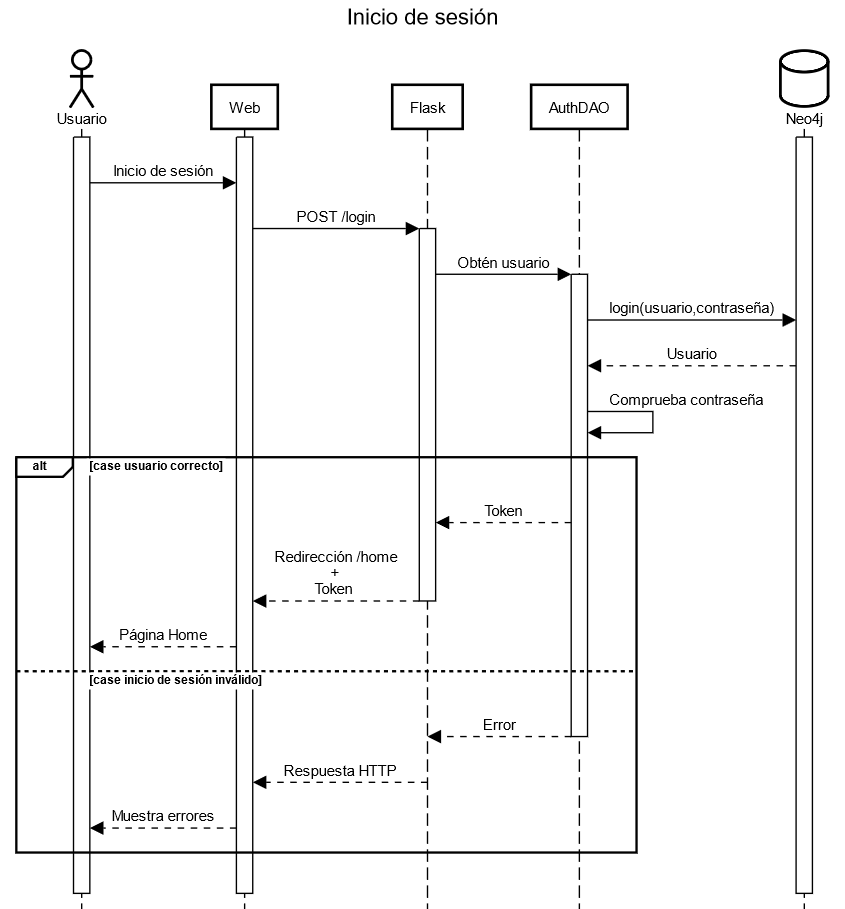
\includegraphics[height=0.8\textheight]{LoginSeq}
	\caption{Diagrama de secuencia de inicio de sesión}\label{LoginSeq}
\end{figure}
\FloatBarrier

\newpage

\subsection{Registro}

	\begin{figure}[!h]
		\centering
		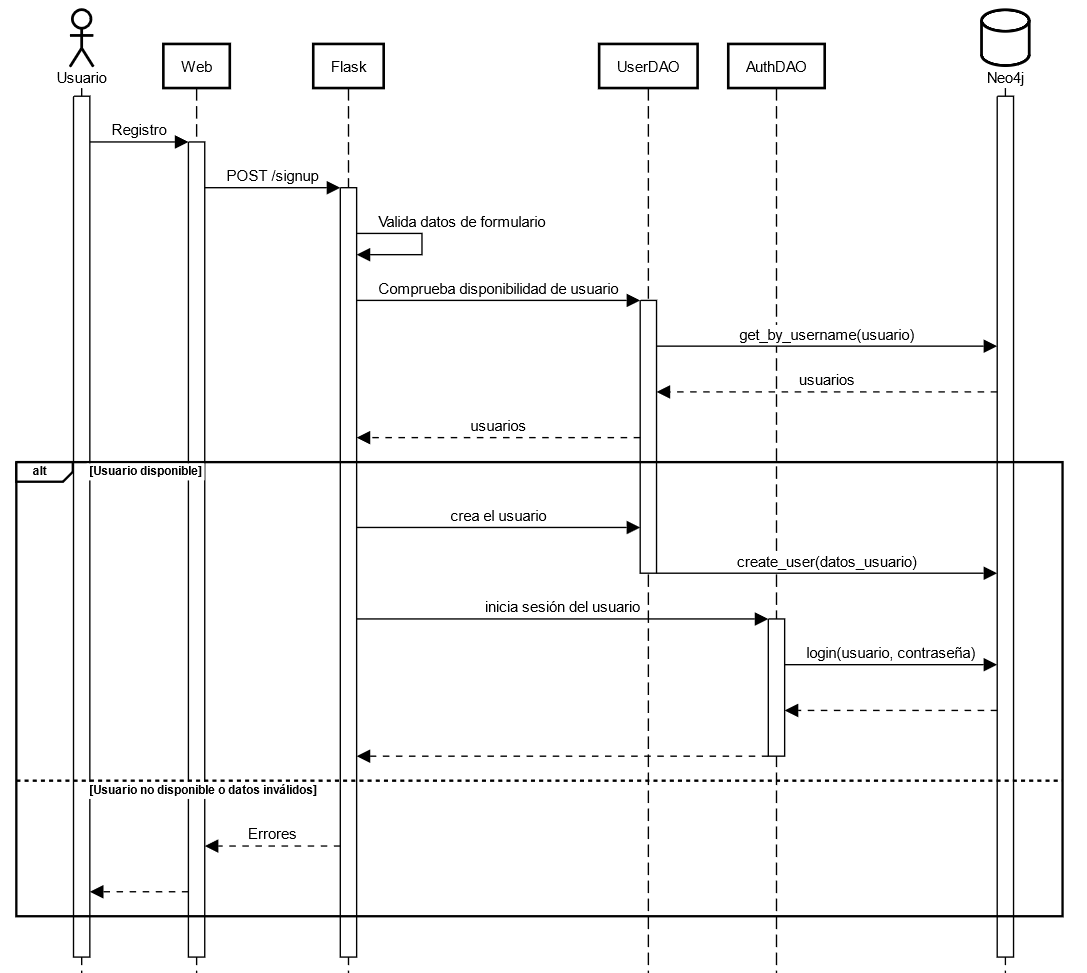
\includegraphics[width=1\textwidth]{SignUpSeq}
		\caption{Diagrama de secuencia de registro}\label{SignUpSeq}
	\end{figure}
	\FloatBarrier

\newpage



\begin{landscape}
	\subsection{Selección de ciudad}
	\begin{figure}[!h]
		\centering
		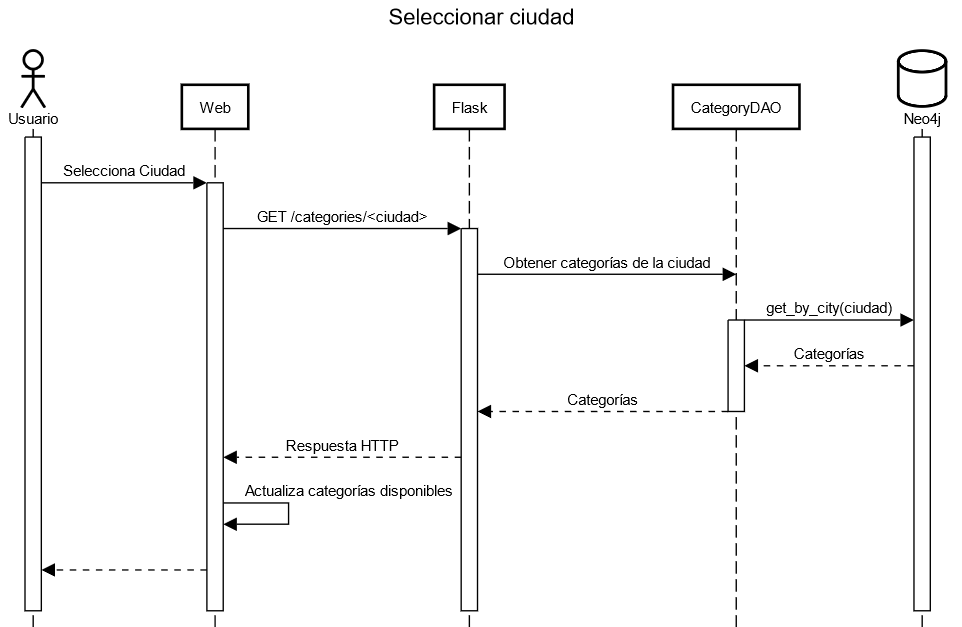
\includegraphics[height=0.8\textheight]{CityCats}
		\caption{Diagrama de secuencia de selección de ciudad}\label{CityCats}
	\end{figure}
	\FloatBarrier
\end{landscape}

\subsection{Recomendaciones de categorías}
	\begin{figure}[!h]
	\centering
	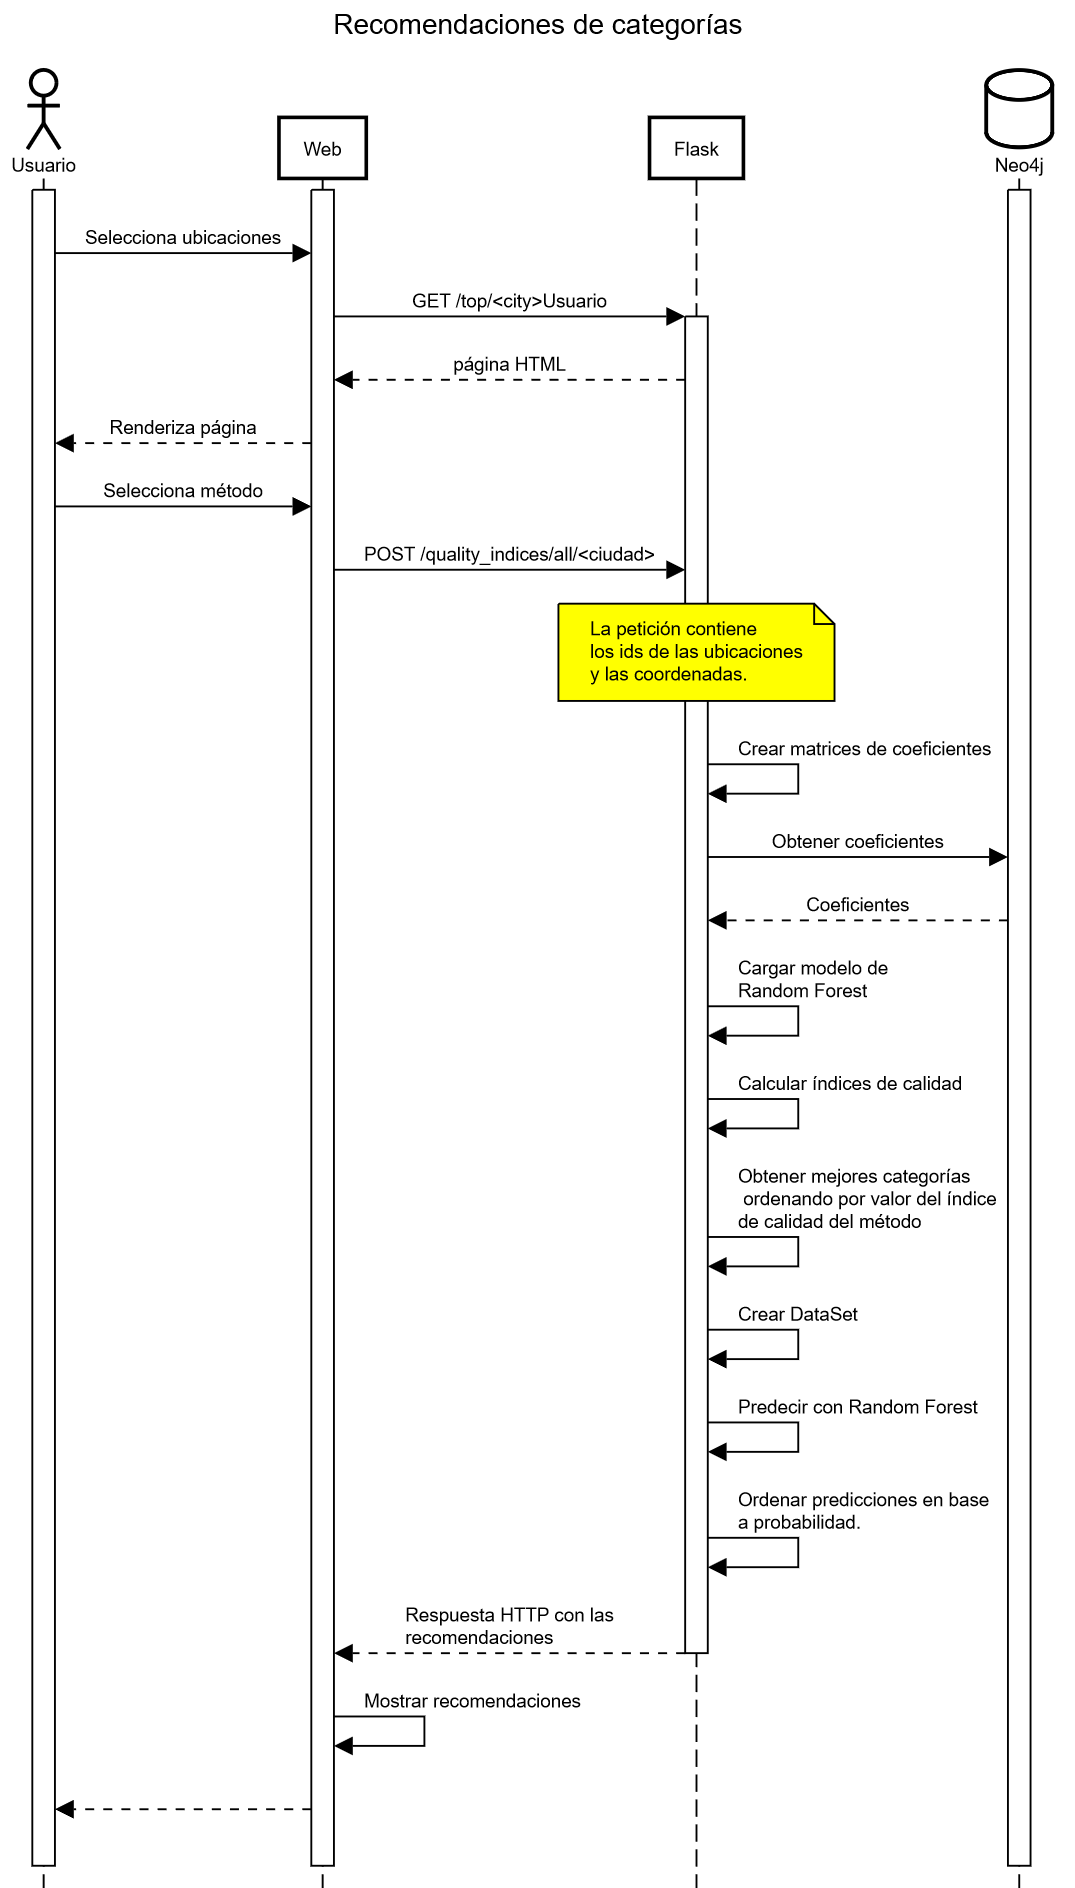
\includegraphics[height=0.8\textheight]{TopsCatsSeq}
	\caption{Diagrama de secuencia de obtención de recomendaciones de categorías}\label{TopsCatsSeq}
\end{figure}
\FloatBarrier
\newpage
\subsection{Recomendaciones de ubicaciones}
	\begin{figure}[!h]
	\centering
	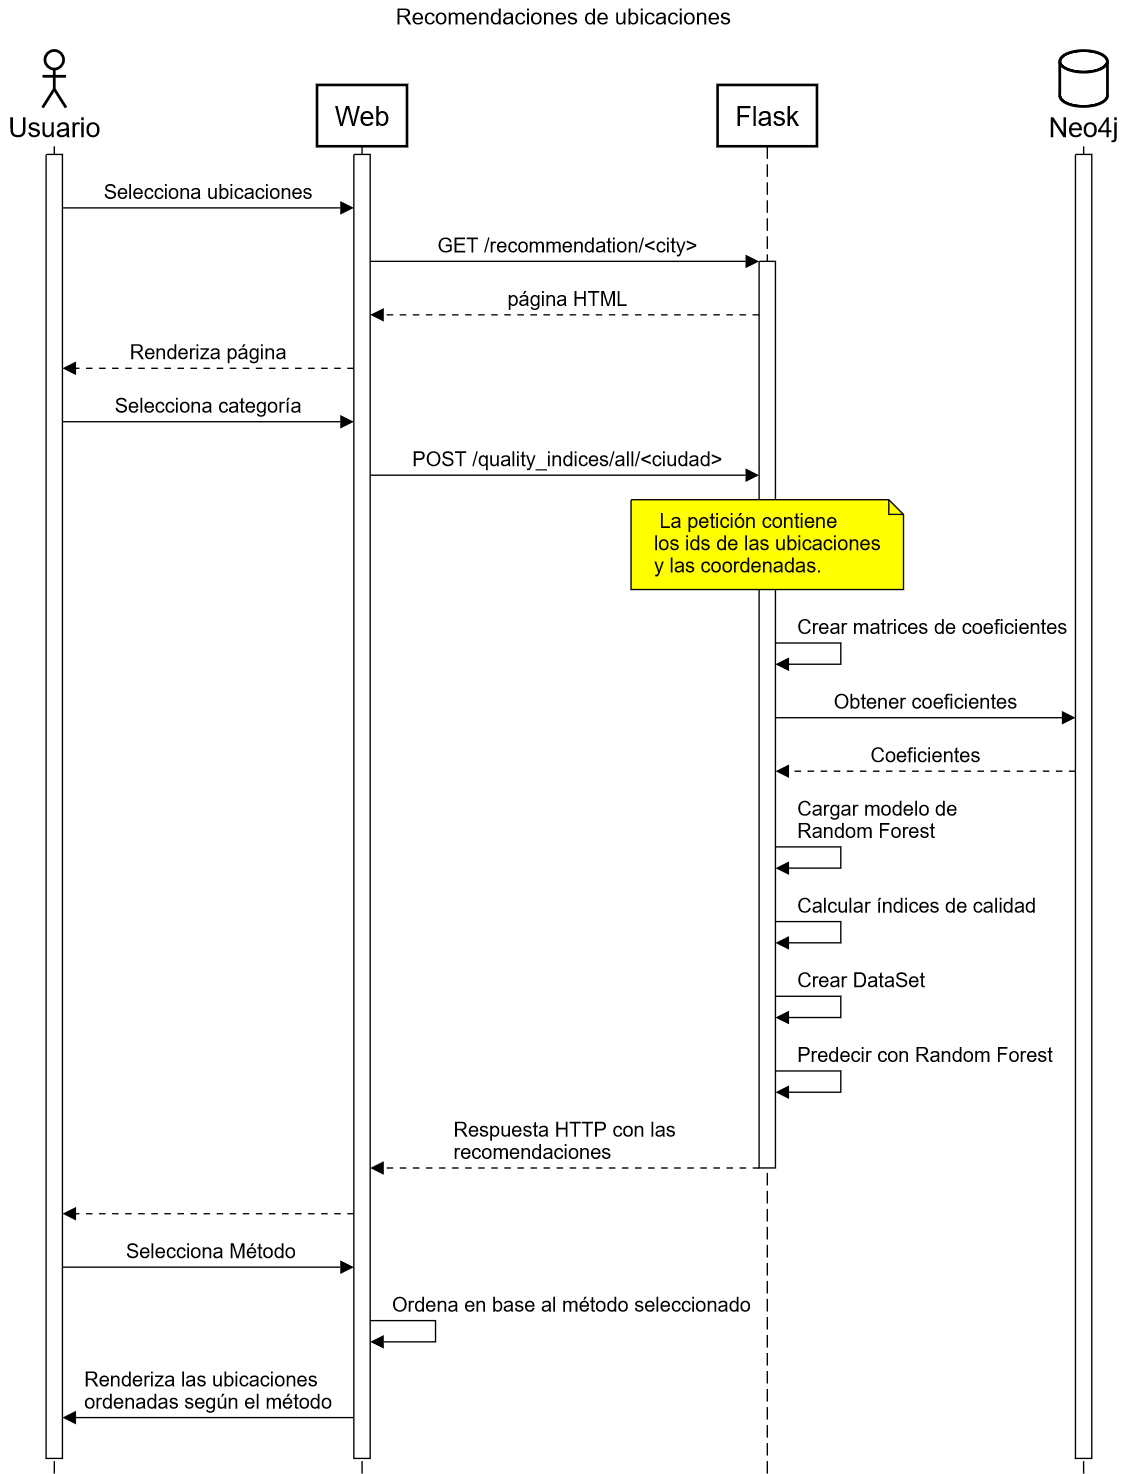
\includegraphics[height=0.8\textheight]{TopsPlacesSeq}
	\caption{Diagrama de secuencia de obtención de recomendaciones de ubicaciones}\label{TopsPlacesSeq}
\end{figure}
\FloatBarrier

\newpage
\subsection{Visualización de red de categorías}
	\begin{figure}[!h]
	\centering
	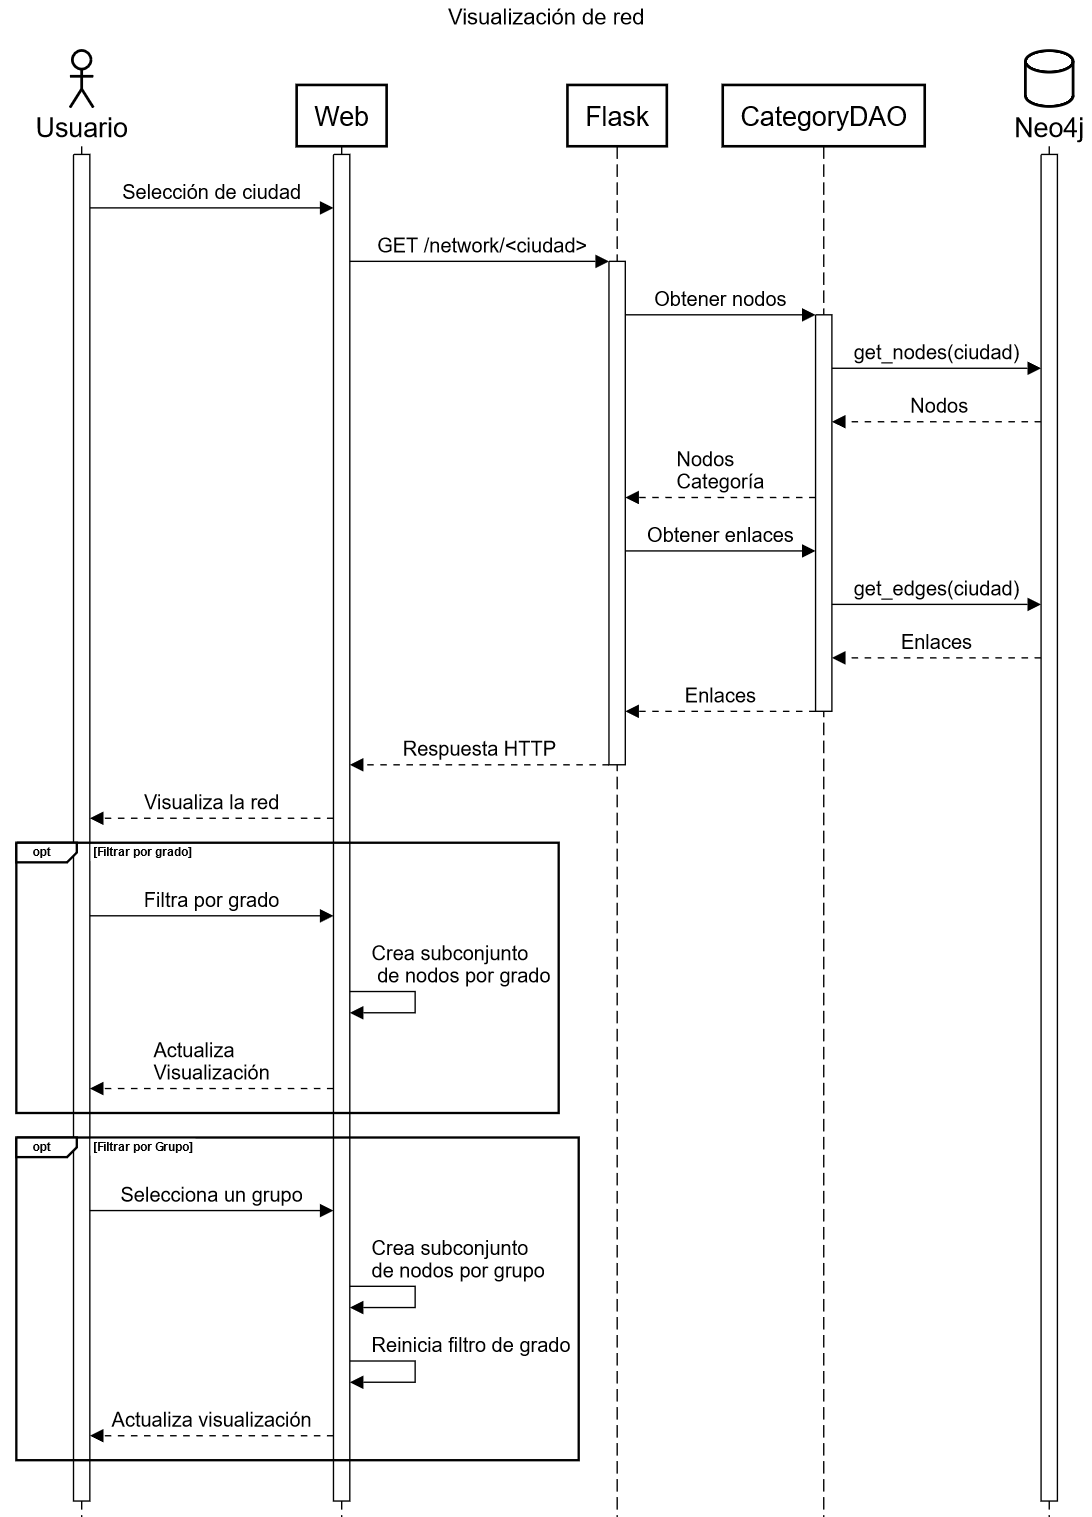
\includegraphics[height=0.8\textheight]{NetworkSeq}
	\caption{Diagrama de secuencia de visualización de red de categorías}\label{NetworkSeq}
\end{figure}
\FloatBarrier
\newpage

\section{Diseño arquitectónico}

Dado que el producto final de este trabajo es una aplicación web conviene mencionar unas estructuras propias de este tipo de aplicaciones.

\subsection{Arquitectura Cliente-Servidor}
La arquitectura cliente servidor es un modelo ampliamente utilizado en el entorno web. Esta está compuesta por dos entidades distintas con diferentes responsabilidades.

\begin{itemize}
	\item Cliente:
	\begin{itemize}
		\item Realiza peticiones al servidor para obtener los recursos o servicios.
		\item Provee una interfaz gráfica al usuario.
		\item Recibe las respuestas del servidor.
	\end{itemize}
	\item Servidor:
	\begin{itemize}
		\item Responde a las peticiones del cliente.
		\item Se encarga de manejar la lógica de negocio y la gestión de recursos.
		\item Puede contar con una conexión con una base de datos en la que puede almacenar y extraer la información requerida.
	\end{itemize}
\end{itemize}

\imagen{ClienteServidor}{Esquema Cliente-Servidor}

En el contexto web y de nuestro proyecto el cliente es el dispositivo desde el que el usuario accede a la aplicación, haciendo peticiones al servidor web mediante el protocolo HTTP. En cuanto al servidor este será el equipo que alojará la aplicación web.
\subsection{Modelo-Vista-Controlador}

El patrón Modelo-Vista-Controlador o MVC se trata de una arquitectura utilizada ampliamente para estructurar proyectos \textit{software}. Esta define 3 distintos componentes con responsabilidades distintas del funcionamiento del programa. Esto permite tener separada la lógica de la aplicación en componentes en base a la responsabilidad que toma, facilitando la organización y futuro mantenimiento.

\imagen{MVC}{Esquema de arquitectura Modelo-Vista-Controlador}

Las partes que componen MVC son las siguientes:
\begin{itemize}
	\item Modelo: El componente Modelo contiene toda la lógica relacionada a los datos, su estructura y manejo. Normalmente interactúa con una base de datos, que es donde aloja la información de la aplicación.
	\item Vista: Es el componente encargado de presentar una interfaz al usuario donde mostrar la información de la aplicación y poder interactuar con esta.
	\item Controlador: Es el componente intermedio entre en el Modelo y la Vista. Se encarga de dar una respuesta adecuada a las entradas del usuario en la Vista e interactuar con el Modelo para modificar la información de la aplicación según la lógica de esta. 
\end{itemize}

Aplicado a nuestro proyecto el componente Modelo se correspondería a los distintos DAOs contenidos en \texttt{/src/web/dao}.

El controlador está compuesto por las distintas rutas definidas en la aplicación Flask en el directorio \texttt{/src/web/routes} junto con la lógica definida en cada uno de ellos para el tratamiento de las peticiones del usuario.

En cuanto a la vista, esta sería todo aquello que se ejecutaría en el lado del servidor, siendo esto plantillas HTML, hojas de estilo y scripts de JavaScript, todo ello contenido dentro del directorio \texttt{/src/web/static}. Esto se corresponde con los ficheros contenidos dentro de \texttt{/templates}, \texttt{/styles} y \texttt{/js} respectivamente. Estas vistas serían aquellas devueltas por las rutas definidas en \texttt{/src/web/routes/views}.